\section{Experimental Results}
\subsection{Example Regression Problem}
This problem serves as a quick example to demonstrate many of the phenomena described in previous sections. We trained two networks to learn the cosine function, with one input and one output. This is a task which requires no more than 11 sigmoid neurons to solve entirely, and in this case we don't care about overfitting because the cosine function has a precise definition. Furthermore, the cosine function is a good toy example because it is a smooth continuous function and, as demonstrated by \cite{nielsen2015neural}, if we were to tinker directly with the weights and bias parameters of the network, we could allocate individual units within the network to be responsible for constrained ranges of inputs, similar to a basis spline function with many control points. This would distribute the learned function approximation evenly across all hidden units, and thus we have presented the network with a problem in which it could productively use as many hidden units as we give it. In this case, a pruning algorithm would observe a fairly consistent increase in error after the removal of each successive unit. In practice however, regardless of the number of experimental trials, this is not what happens. The network will always use 10-11 hidden units and leave the rest to cancel each other's influence.

\begin{figure}[!h]
\centering
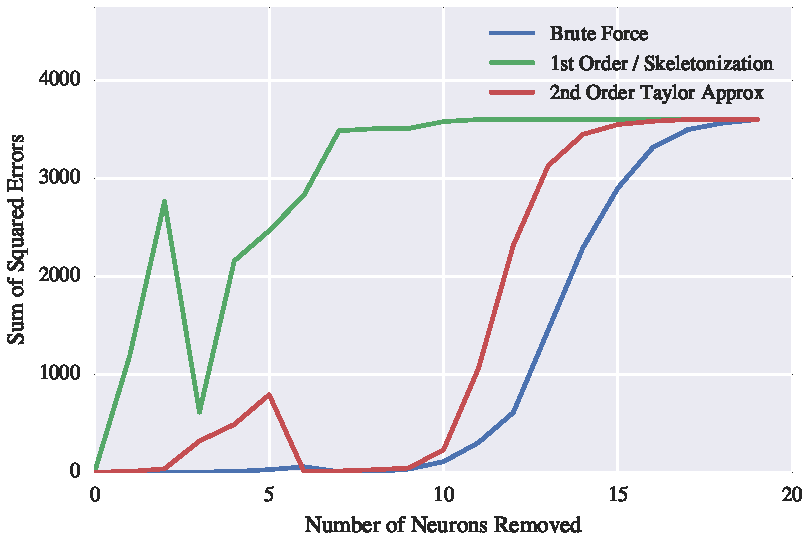
\includegraphics[width=0.49\linewidth]{png/cos-small.pdf}
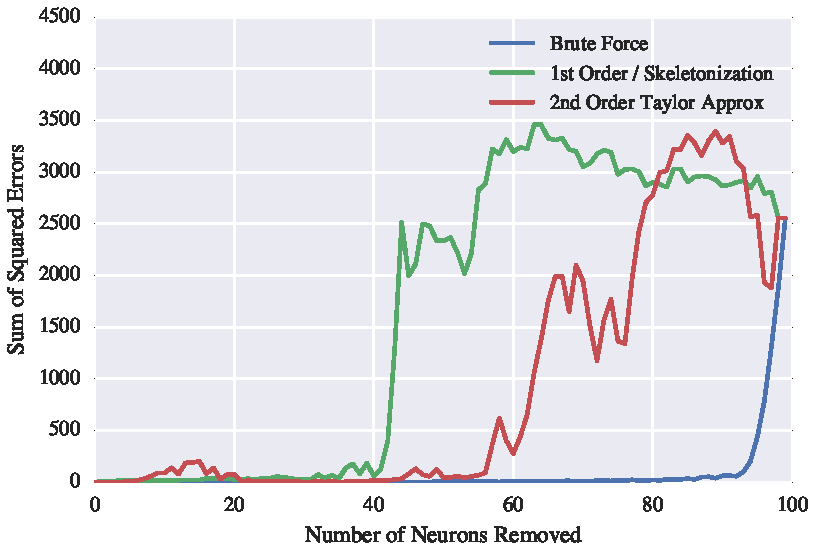
\includegraphics[width=0.49\linewidth]{png/cos-big.pdf}
\caption{Degradation in squared error after pruning a two-layer network trained to compute the cosine function (\textbf{Left Network:} 2 layers, 10 neurons each, 1 output, logistic sigmoid activation, starting test accuracy: 0.9999993, \textbf{Right Network:} 2 layers, 50 neurons each, 1 output, logistic sigmoid activation, starting test accuracy: 0.9999996)}
\label{fig:cosine-double-layer}
\end{figure}

Figure \ref{fig:cosine-double-layer} shows two graphs. Both graphs demonstrate the use of the iterative re-ranking algorithm and the comparative performance of the brute-force pruning method (in blue), the first order method (in green), and the second order method (in red). The graph on the left shows the performance of these algorithms starting from a network with two layers of 10 neurons (20 total), and the graph on the right shows a network with two layers of 50 neurons (100 total). 

In the left graph, we see that the brute-force method shows a graceful degradation, and the error only begins to rise sharply after 50\% of the total neurons have been removed. The error is basically constant up to that point. In the first and second order methods, we see evidence of poor decision making in the sense that both made mistakes early on, which disrupted the output function approximation. The first order method made a large error early on, though we see after a few more neurons were removed this error was corrected somewhat (though it only got worse from there). This is direct evidence of the lack of fault tolerance in a trained neural network. This phenomenon is even more starkly demonstrated in the second order method. After making a few poor neuron removal decisions in a row, the error signal rose sharply, and then went back to zero after the 6th neuron was removed. This is due to the fact that the neurons it chose to remove were trained to cancel each others' influence within a localized part of the network. After the entire group was eliminated, the approximation returned to normal. This can only happen if the output function approximation is not evenly distributed over the hidden units in a trained network. 

This phenomenon is even more starkly demonstrated in the graph on the right. Here we see the first order method got ``lucky'' in the beginning and made decent decisions up to about the 40th removed neuron. The second order method had a small error in the beginning which it recovered from gracefully and proceeded to pass the 50 neuron point before finally beginning to unravel. The brute force method, in sharp contrast, shows little to no increase in error at all until 90\% of the neurons in the network have been obliterated. Clearly first and second order methods have some value in that they do not make completely arbitrary choices, but the brute force method is far better at this task. 

This also demonstrates the sharp dualism in neuron roles within a trained network. These networks were trained to near-perfect precision and each pruning method was applied \textit{without} any re-training of any kind. Clearly, in the case of the brute force or oracle method, up to 90\% of the network can be completely extirpated before the output approximation even begins to show any signs of degradation. This would be impossible if the learning representation were evenly or equitably distributed. Note, for example, that the degradation point in both cases is approximately the same. This example is not a real-world application of course, but it brings into very clear focus the kind of phenomena we will discuss in the following sections. 

\subsection{Results on MNIST Dataset}
For all the results presented in this section, the MNIST database of Handwritten Digits by \cite{lecun-mnisthandwrittendigit-2010} was used. It is worth noting that due to the time taken by the brute force algorithm we rather used a 5000 image subset of the MNIST database in which we have normalized the pixel values between 0 and 1.0, and compressed the image sizes to 20x20 images rather than 28x28, so the starting test accuracy reported here appears higher than those reported by LeCun et al. We do not believe that this affects the interpretation of the presented results because the basic learning problem does not change with a larger dataset or input dimension.

\subsection{Pruning a 1-Layer Network}
The network architecture in this case consisted of 1 layer, 100 neurons, 10 outputs, logistic sigmoid activations, and a starting test accuracy of 0.998.

\subsubsection{Single Overall Ranking Algorithm}
We first present the results for a single-layer neural network in Figure \ref{fig:mnist-single-ranking-single-layer}, using the Single Overall algorithm (Algorithm \ref{algo1}) as proposed in Section \ref{sec2}. (We again note that this algorithm is intentionally naive and is used for comparison only. Its performance should be expected to be poor.) After training, each neuron is assigned its permanent ranking based on the three criteria discussed previously: A brute force ``ground truth'' ranking, and two approximations of this ranking using first and second order Taylor estimations of the change in network output error resulting from the removal of each neuron. 

\begin{figure}[!h]
\centering
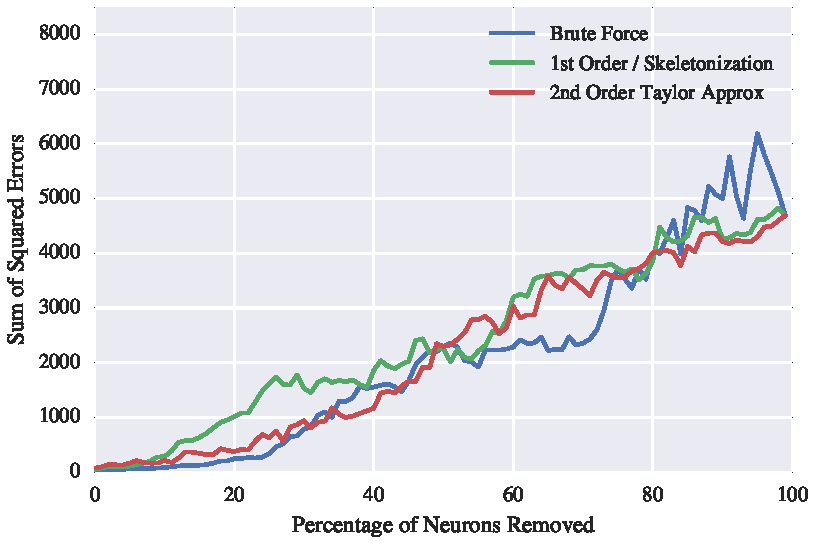
\includegraphics[width=0.49\linewidth]{png/mnist-acc99-single-pass-method.pdf}
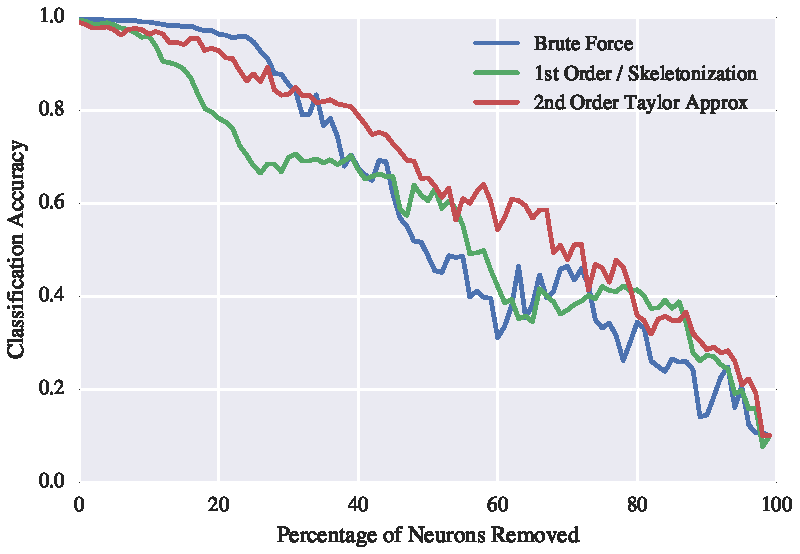
\includegraphics[width=0.49\linewidth]{png/mnist-acc99-single-pass-accuracy.pdf}
\caption{Degradation in squared error (left) and classification accuracy (right) after pruning a single-layer network using The Single Overall Ranking algorithm (\textbf{Network:} 1 layer, 100 neurons, 10 outputs, logistic sigmoid activation, starting test accuracy: 0.998)}
\label{fig:mnist-single-ranking-single-layer}
\end{figure}

An interesting observation here is that with only a single layer, no criteria for ranking the neurons in the network (brute force or the two Taylor Series variants) using Algorithm \ref{algo1} emerges superior, indicating that the 1st and 2nd order Taylor Series methods are actually reasonable approximations of the brute force method under certain conditions. Of course, this method is still quite bad in terms of the rate of degradation of the classification accuracy and in practice we would likely follow Algorithm \ref{algo2} which is takes into account \cite{mozer1989skeletonization}'s observations stated in the Related Work section. The purpose of the present investigation, however, is to demonstrate how much of a trained network can be theoretically removed without altering the network's learned parameters in any way.

\subsubsection{Iterative Re-Ranking Algorithm}

\begin{figure}[!hb]
\centering
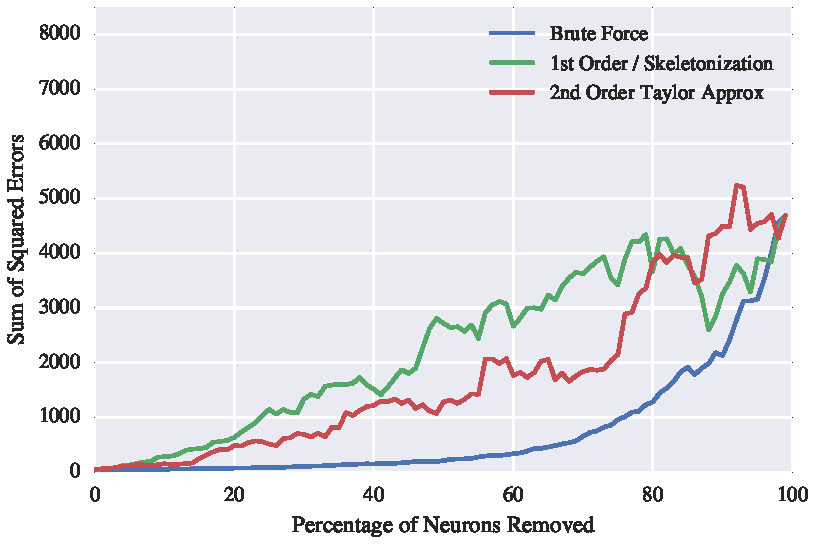
\includegraphics[width=0.49\linewidth]{png/mnist-acc99-iterative-rerank-method.pdf}
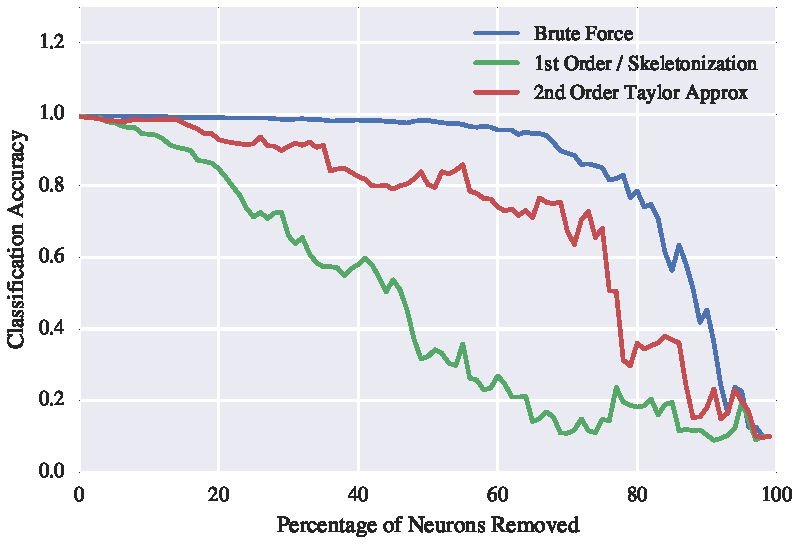
\includegraphics[width=0.49\linewidth]{png/mnist-acc99-iterative-rerank-accuracy.pdf}
\caption{Degradation in squared error (left) and classification accuracy (right) after pruning a single-layer network the Iterative Re-ranking algorithm (\textbf{Network:} 1 layer, 100 neurons, 10 outputs, logistic sigmoid activation, starting test accuracy: 0.998)}
\label{fig:mnist-re-ranking-single-layer}
\end{figure}

In Figure \ref{fig:mnist-re-ranking-single-layer} we present our results using Algorithm \ref{algo2} (The Iterative Re-Ranking Algorithm) in which all remaining neurons are re-ranked after each successive neuron is switched off. We compute the same brute force rankings and Taylor series approximations of error deltas over the remaining active neurons in the network after each pruning decision. This is intended to account for the effects of cancelling interactions between neurons. 

There are 2 key observations here. Using the Brute Force ranking criteria, almost 60\% of the neurons in the network can be pruned away without any major loss in performance. The other noteworthy observation here is that the 2nd order Taylor Series approximation of the error performs consistently better than its 1st order version.

%tl;dr: 1 layer is grrrreat for brute force! Clearly 2nd order method is consistently better than 1st order method. 

%tl;dr: Brute force method is amazing here! 1 layer makes things a lot easier, and a 2nd order method can do okay as well, but can still be improved a lot. 60% of neurons doing nothing!

\subsubsection{Visualization of Error Surface \& Pruning Decisions}

\begin{figure}[!hb]
\centering
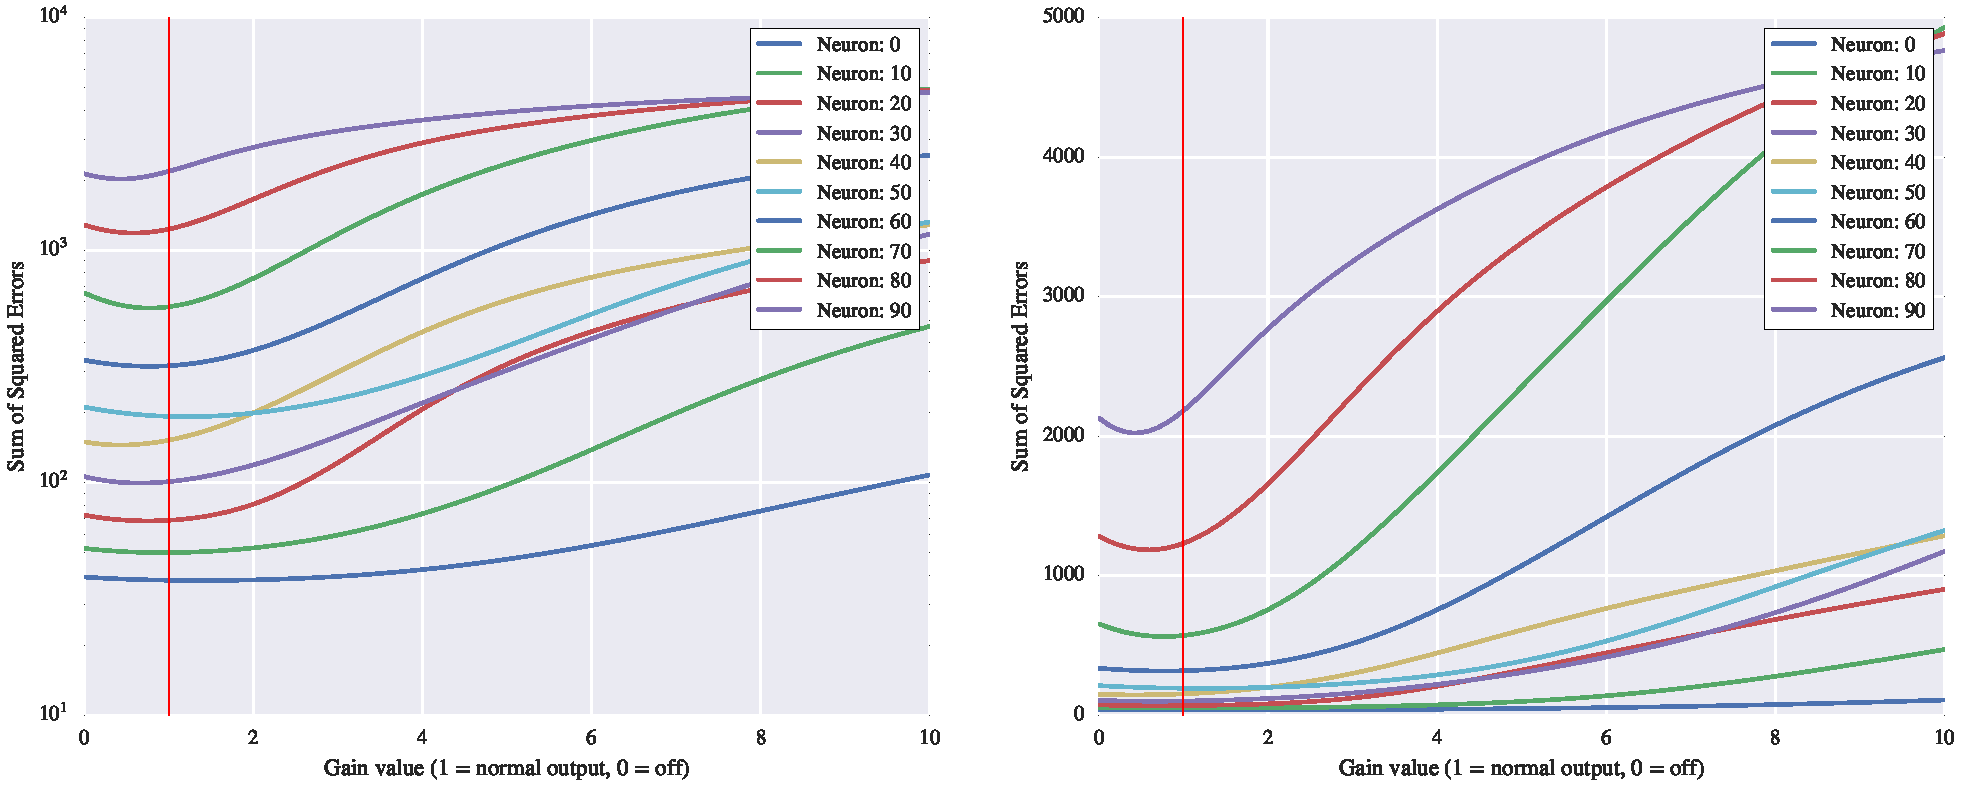
\includegraphics[width=\linewidth]{png/mnist-acc99-gt-gain.pdf}
\caption{Error surface of the network output in log space (left) and in real space (right) with respect to each candidate neuron chosen for removal using the brute force criterion; (\textbf{Network:} 1 layer, 100 neurons, 10 outputs, logistic sigmoid activation, starting test accuracy: 0.998)}
\label{fig:mnist-gt-single-layer}
\end{figure}

\begin{figure}[!hb]
\centering
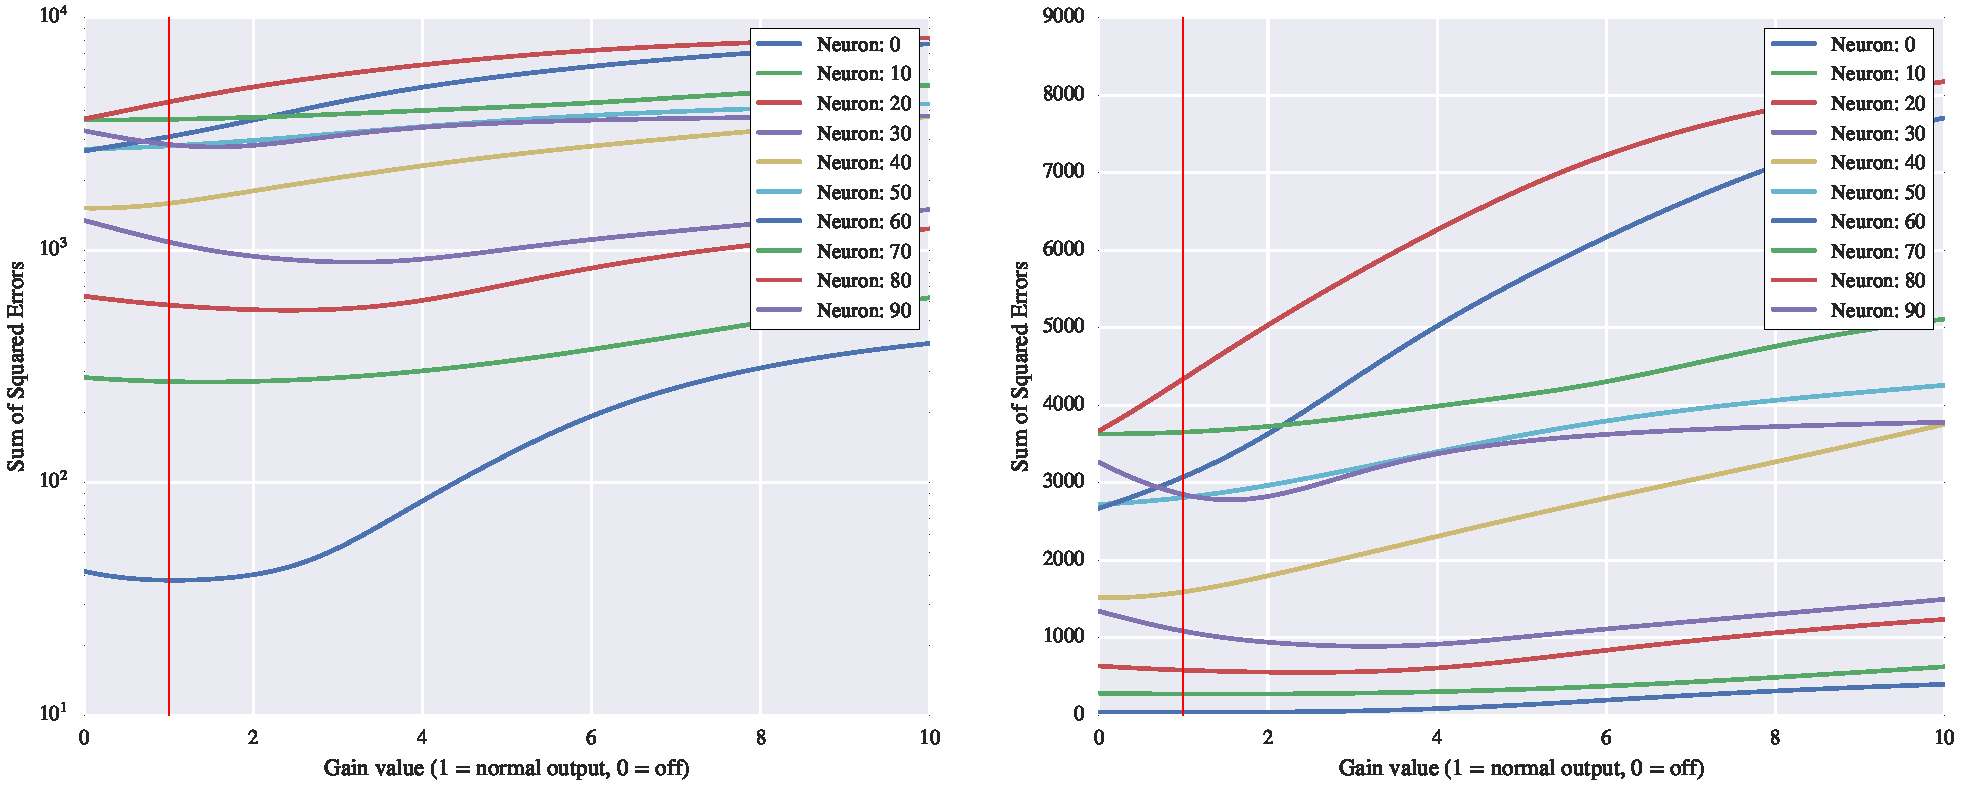
\includegraphics[width=\linewidth]{png/mnist-acc99-g1-gain.pdf}
\caption{Error surface of the network output in log space (left) and in real space (right) with respect to each candidate neuron chosen for removal using the 1st order Taylor Series error approximation criterion; (\textbf{Network:} 1 layer, 100 neurons, 10 outputs, logistic sigmoid activation, starting test accuracy: 0.998)}
\label{fig:mnist-gt-single-layer}
\end{figure}

\begin{figure}[!hb]
\centering
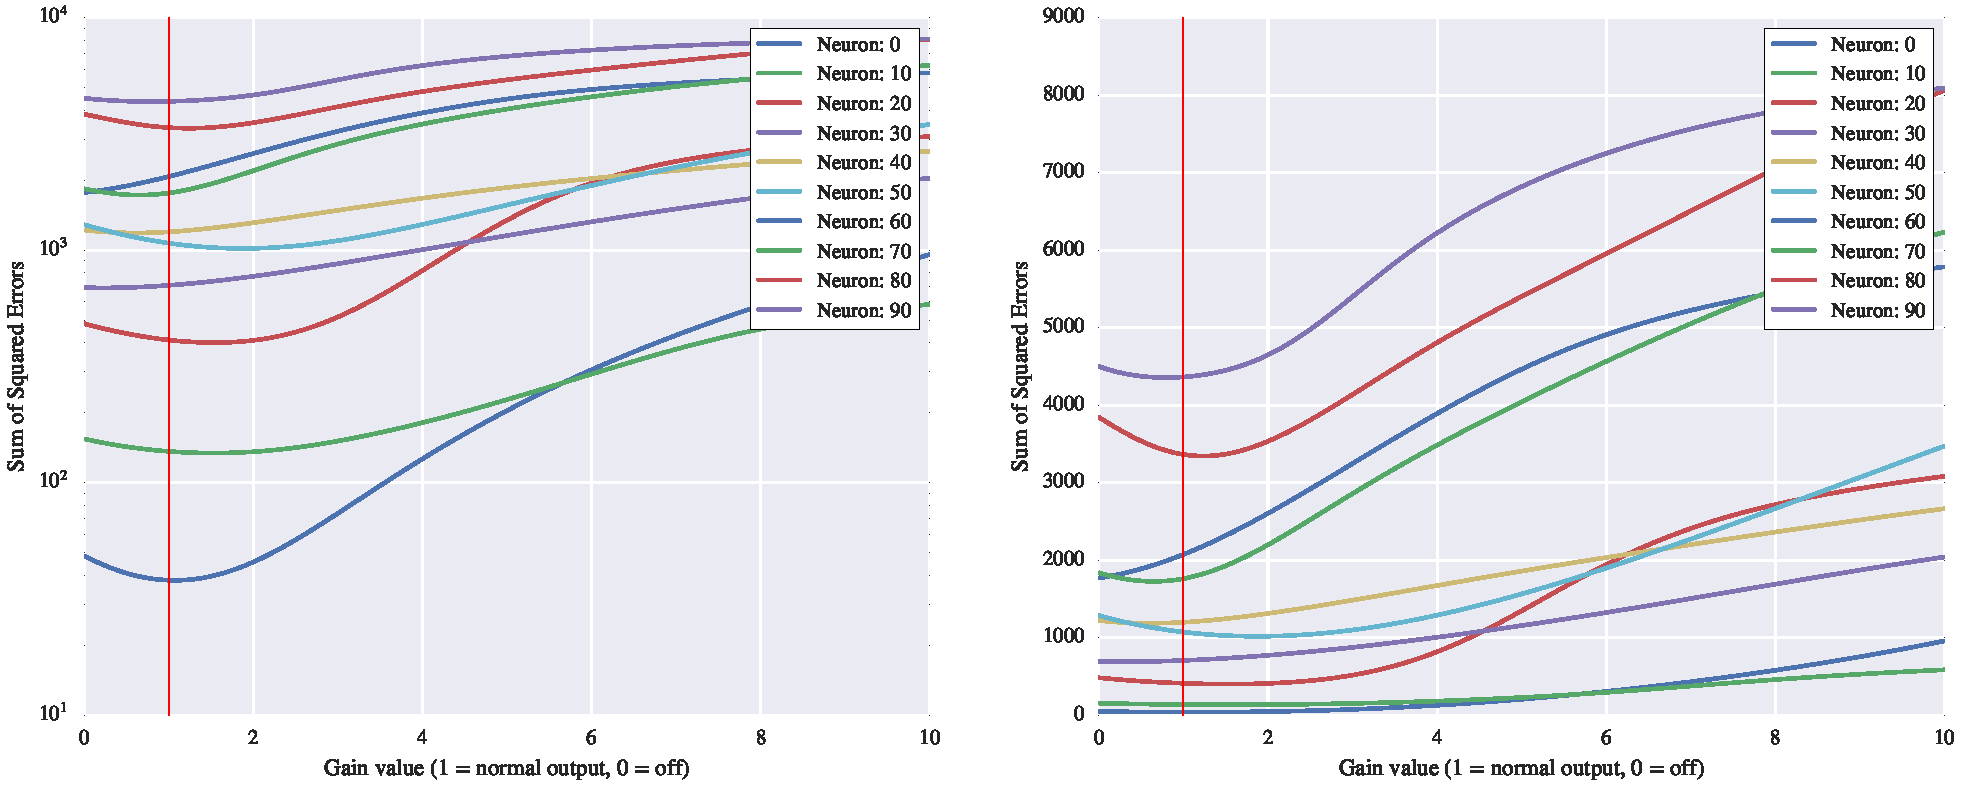
\includegraphics[width=\linewidth]{png/mnist-acc99-g2-gain.pdf}
\caption{Error surface of the network output in log space (left) and in real space (right) with respect to each candidate neuron chosen for removal using the 2nd order Taylor Series error approximation criterion; (\textbf{Network:} 1 layer, 100 neurons, 10 outputs, logistic sigmoid activation, starting test accuracy: 0.998)}
\label{fig:mnist-gt-single-layer}
\end{figure}

As explained in Section \ref{sec2}, these graphs are a visualization of the error surface of the network output with respect to the neurons chosen for removal using each of the 3 ranking criteria, represented in intervals of 10 neurons. In each graph, the error surface of the network output is displayed in log space (left) and in real space (right) with respect to each candidate neuron chosen for removal. We create these plots during the pruning exercise by picking a neuron to switch off, and then multiplying its output by a scalar gain value $\alpha$ which is adjusted from 0.0 to 10.0 with a step size of 0.001. When the value of $\alpha$ is 1.0, this represents the unperturbed neuron output learned during training. Between 0.0 and 1.0, we are graphing the literal effect of turning the neuron off ($\alpha = 0$), and when $\alpha > 1.0$ we are simulating a boosting of the neuron's influence in the network, i.e. inflating the value of its outgoing weight parameters. 

We graph the effect of boosting the neuron's output to demonstrate that for certain neurons in the network, even doubling, tripling, or quadrupling the scalar output of the neuron has no effect on the overall error of the network, indicating the remarkable degree to which the network has learned to ignore the value of certain parameters. In other cases, we can get a sense of the sensitivity of the network's output to the value of a given neuron when the curve rises steeply after the red 1.0 line. This indicates that the learned value of the parameters emanating from a given neuron are relatively important, and this is why we should ideally see sharper upticks in the curves for the later-removed neurons in the network, that is, when the neurons crucial to the learning representation start to be picked off. 

%Remember that lower is better in terms of the height of the curve and minimal horizontal change between the vertical red line at 1.0 (neuron \textit{on}, $\alpha = 1.0$) and 0.0 (neuron \textit{off}, $\alpha = 0.0$) is indicative of a good candidate neuron to prune, i.e. there will be minimal effect on the network output when the neuron is removed. 

Some very interesting observations can be made in each of these graphs.

\textbf{Brute Force Criterion}

Notice how low to the floor and flat most of these curves are. It's only until the 90th removed neuron that we see a higher curve with a more convex shape (clearly a more influential piece of the network). This again validates the fact that a good majority of the neurons in a network do not contribute to the overall performance. 

\textbf{1st Order Approximation Criterion}

It can be seen that most choices seem to have flat or negatively sloped curves, indicating that the first order approximation seems to be pretty good, but examining the brute force choices shows they could be better. 

\textbf{2nd Order Approximation Criterion}

This method looks much more similar to the Brute Force method choices, though clearly not as good (they're more spread out). Notice the difference in convexity between the 2nd and 1st order method choices. It's clear that the first order method is fitting a line and the 2nd order method is fitting a parabola in their approximation. 

\subsection{Pruning A 2-Layer Network}
The network architecture in this case consisted of 2 layers, 50 neurons per layer, 10 outputs, logistic sigmoid activations, and a starting test accuracy of 1.000.
\subsubsection{Single Overall Ranking Algorithm}

\begin{figure}[!hb]
\centering
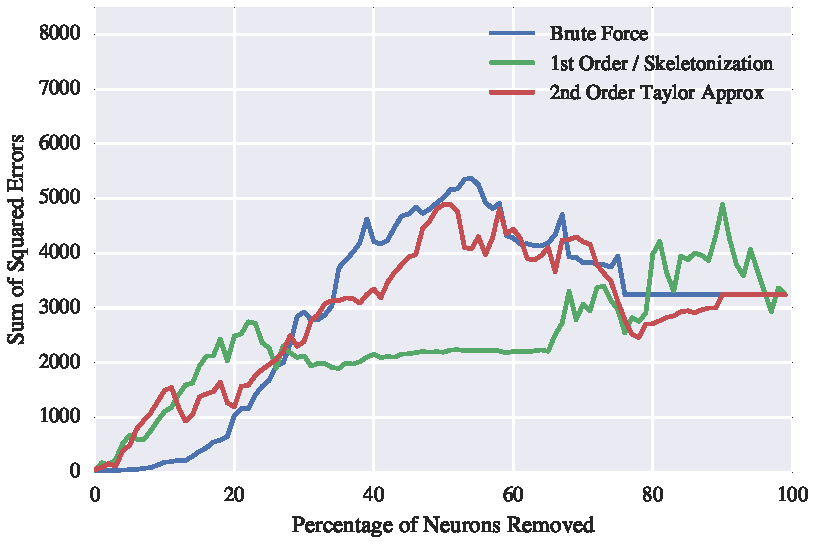
\includegraphics[width=0.49\linewidth]{png/mnist-deep-single-pass-method.pdf}
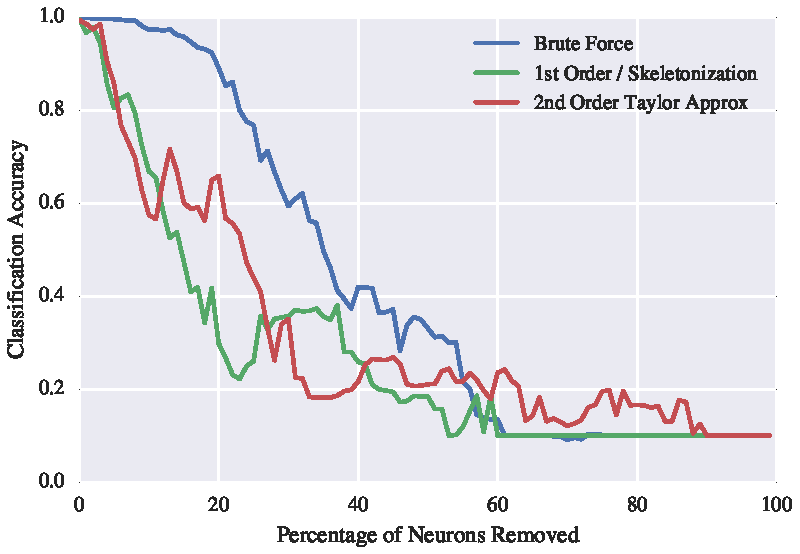
\includegraphics[width=0.49\linewidth]{png/mnist-deep-single-pass-accuracy.pdf}
\caption{Degradation in squared error (left) and classification accuracy (right) after pruning a 2-layer network using the Single Overall Ranking algorithm; (\textbf{Network:} 2 layers, 50 neurons/layer, 10 outputs, logistic sigmoid activation, starting test accuracy: 1.000)}
\label{fig:mnist-single-ranking-double-layer}
\end{figure}

Figure \ref{fig:mnist-single-ranking-double-layer} shows the pruning results for Algorithm \ref{algo1} on a 2-layer network. The ranking procedure is identical to the one used to generate Figure \ref{fig:mnist-single-ranking-single-layer}. (We again note that this algorithm is intentionally naive and is used for comparison only. Its performance should be expected to be poor.) 

Unsurprisingly, a 2-layer network is harder to prune because a single overall ranking will never capture the interdependencies between neurons in different layers. It makes sense that this is much worse than the performance on the 1-layer network, even if this method is already known to be bad, and we'd likely never use it in practice. 


\subsubsection{Iterative Re-Ranking Algorithm}

\begin{figure}[!hb]
\centering
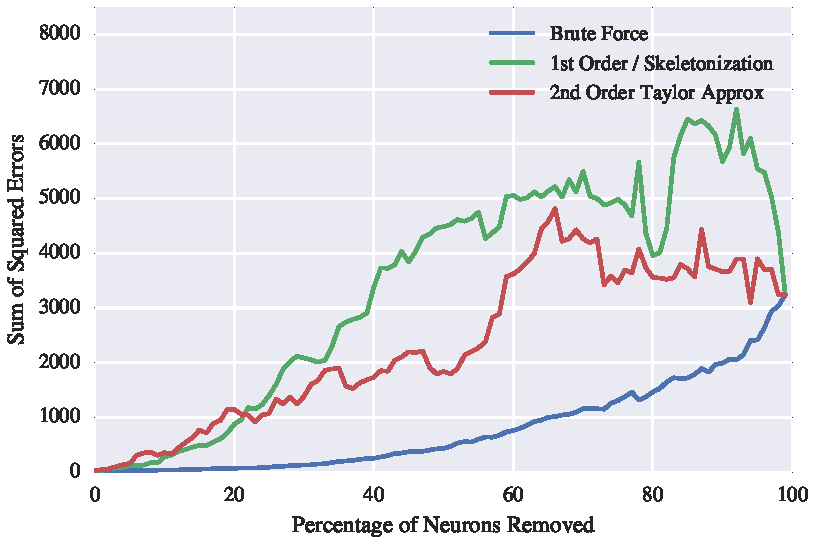
\includegraphics[width=0.49\linewidth]{png/mnist-deep-iterative-rerank-method.pdf}
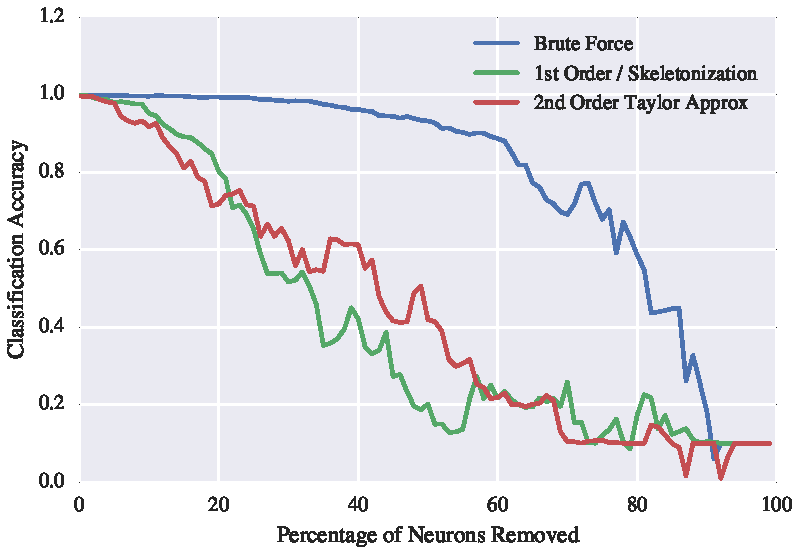
\includegraphics[width=0.49\linewidth]{png/mnist-deep-iterative-rerank-accuracy.pdf}
\caption{Degradation in squared error (left) and classification accuracy (right) after pruning a 2-layer network using the Iterative Re-ranking algorithm; (\textbf{Network:} 2 layers, 50 neurons/layer, 10 outputs, logistic sigmoid activation, starting test accuracy: 1.000)}
\label{fig:mnist-re-ranking-double-layer}
\end{figure}

Figure \ref{fig:mnist-re-ranking-double-layer} shows the results from using Algorithm \ref{algo2} on a 2-layer network. We compute the same brute force rankings and Taylor series approximations of error deltas over the remaining active neurons in the network after each pruning decision used to generate Figure \ref{fig:mnist-re-ranking-single-layer}. Again, this is intended to account for the effects of cancelling interactions between neurons. 

It is clear that it becomes harder to remove neurons 1-by-1 with a deeper network (which makes sense because the neurons have more interdependencies in a deeper network), but we see an overall better performance with 2nd order method vs. 1st order, except for the first 20\% of the neurons (but this doesn't seem to make much difference for classification accuracy.) 

Perhaps a more important observation here is that even with a more complex network, it is possible to remove up to 40\% of the neurons with no major loss in performance which is clearly illustrated by the brute force curve. This shows the clear potential of an ideal pruning technique and also shows how inconsistent 1st and 2nd order Taylor Series approximations of the error can be as ranking criteria.

\subsubsection{Visualization of Error Surface \& Pruning Decisions}

\begin{figure}[!hb]
\centering
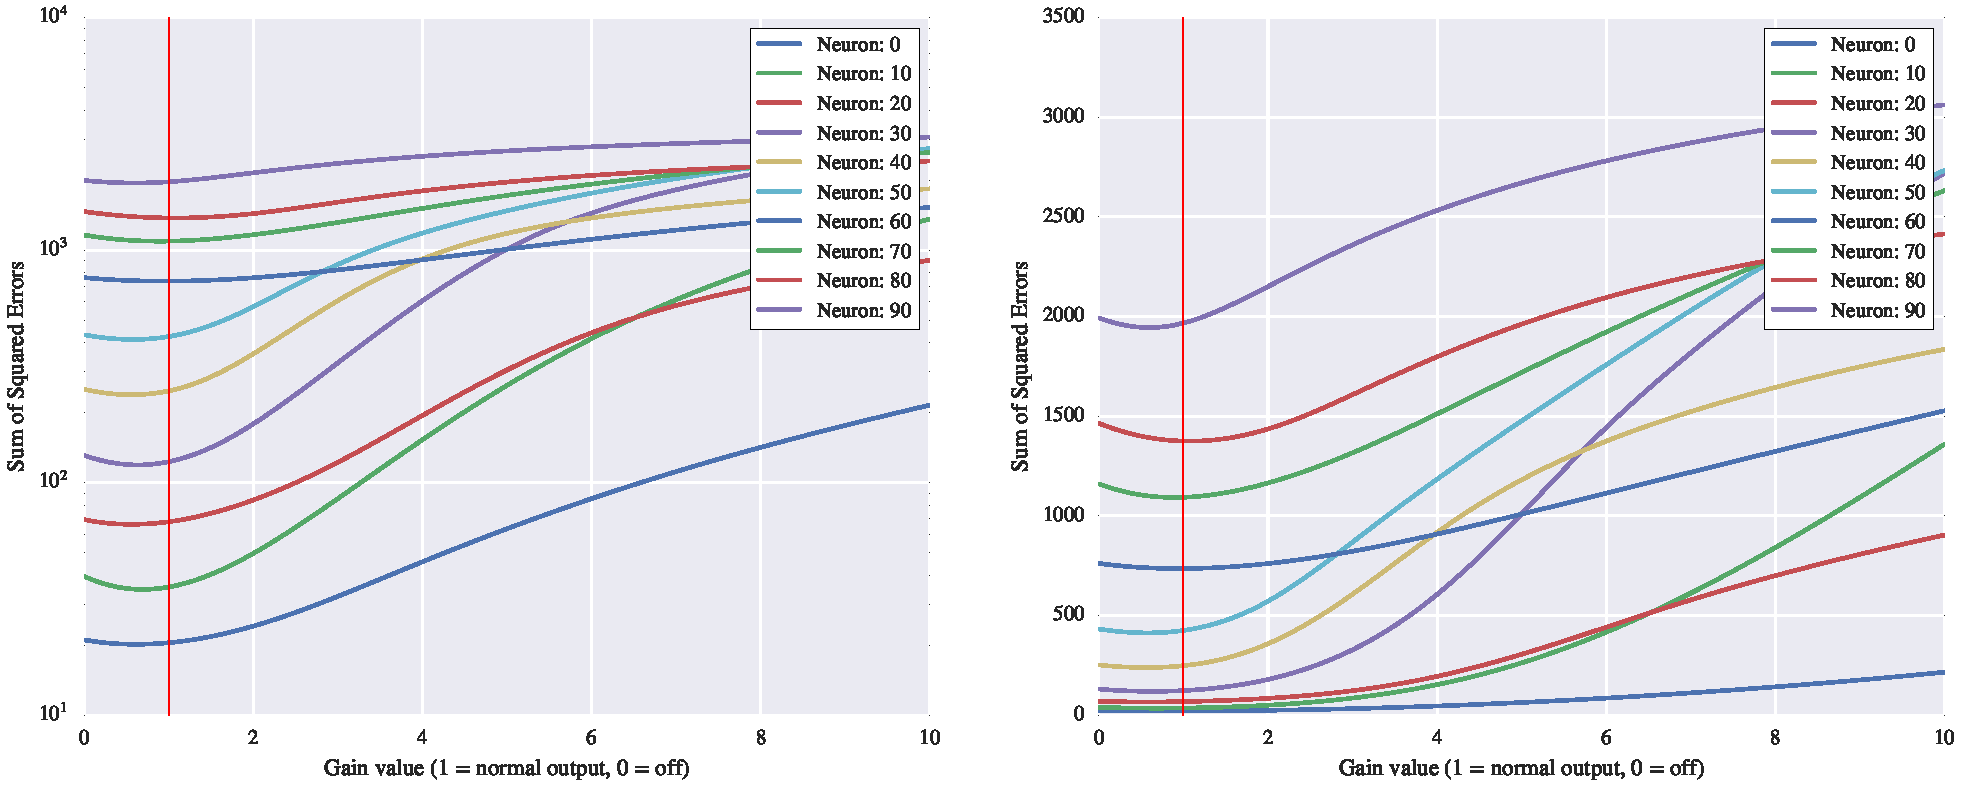
\includegraphics[width=\linewidth]{png/mnist-deep-gt-gain.pdf}
\caption{Error surface of the network output in log space (left) and in real space (right) with respect to each candidate neuron chosen for removal using the brute force criterion; (\textbf{Network:} 2 layers, 50 neurons/layer, 10 outputs, logistic sigmoid activation, starting test accuracy: 1.000)}
\label{fig:mnist-gt-double-layer}
\end{figure}

\begin{figure}[!hb]
\centering
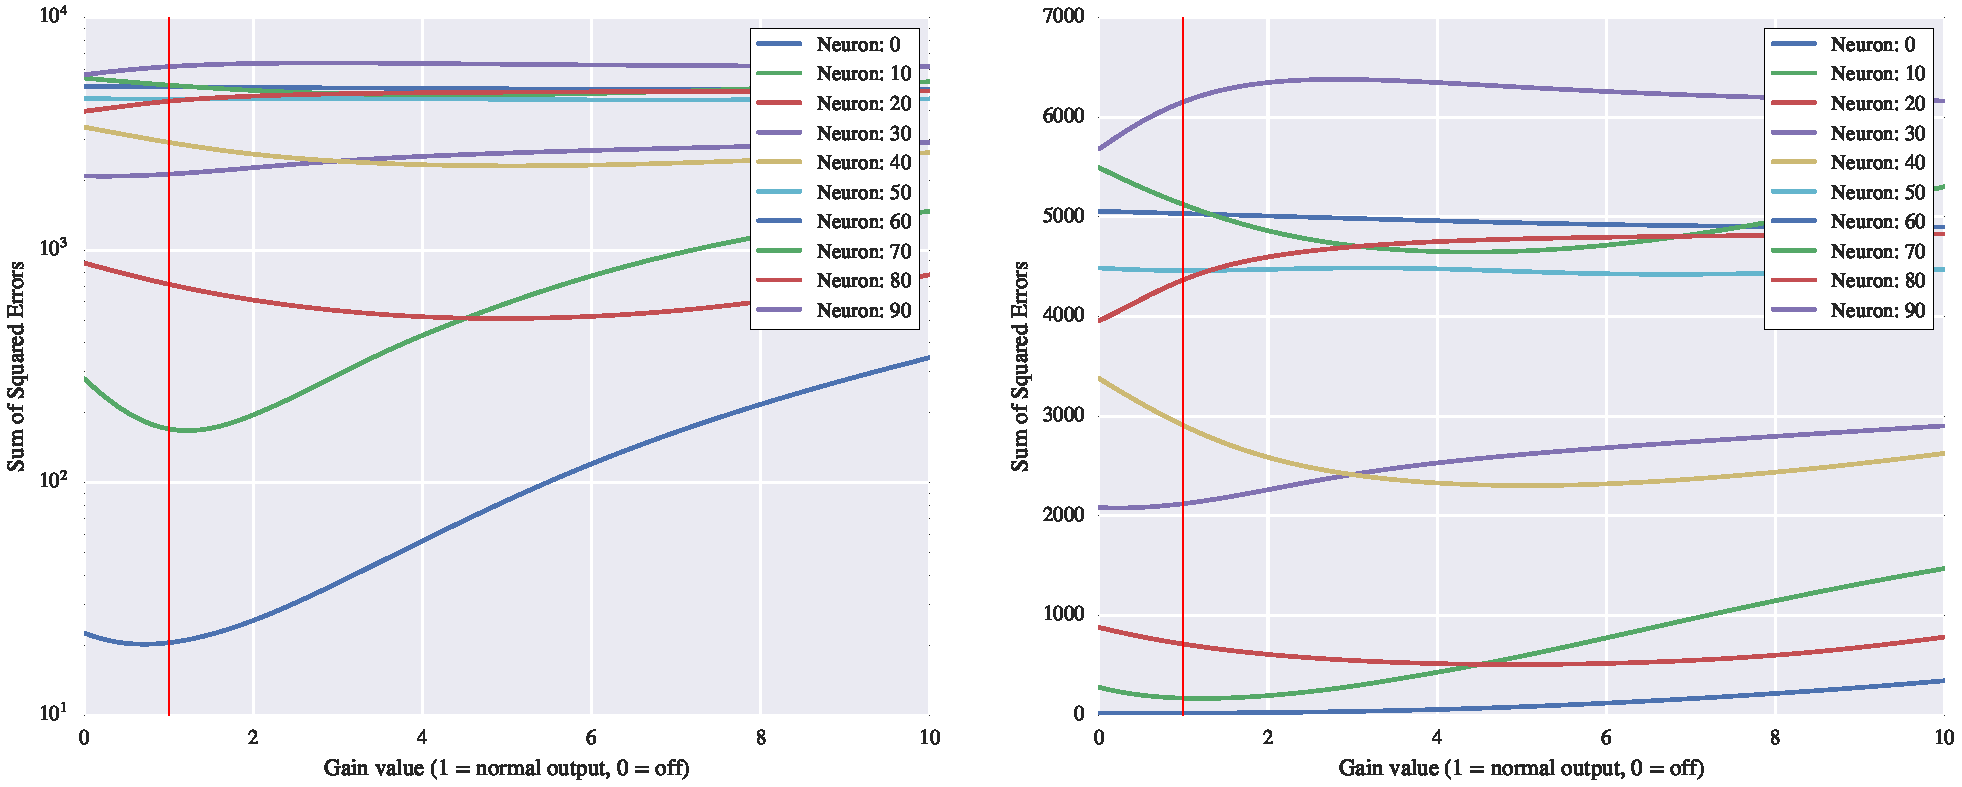
\includegraphics[width=\linewidth]{png/mnist-deep-g1-gain.pdf}
\caption{Error surface of the network output in log space (left) and in real space (right) with respect to each candidate neuron chosen for removal using the 1st order Taylor Series error approximation criterion; (\textbf{Network:} 2 layers, 50 neurons/layer, 10 outputs, logistic sigmoid activation, starting test accuracy: 1.000)}
\label{fig:mnist-g1-double-layer}
\end{figure}

\begin{figure}[!hb]
\centering
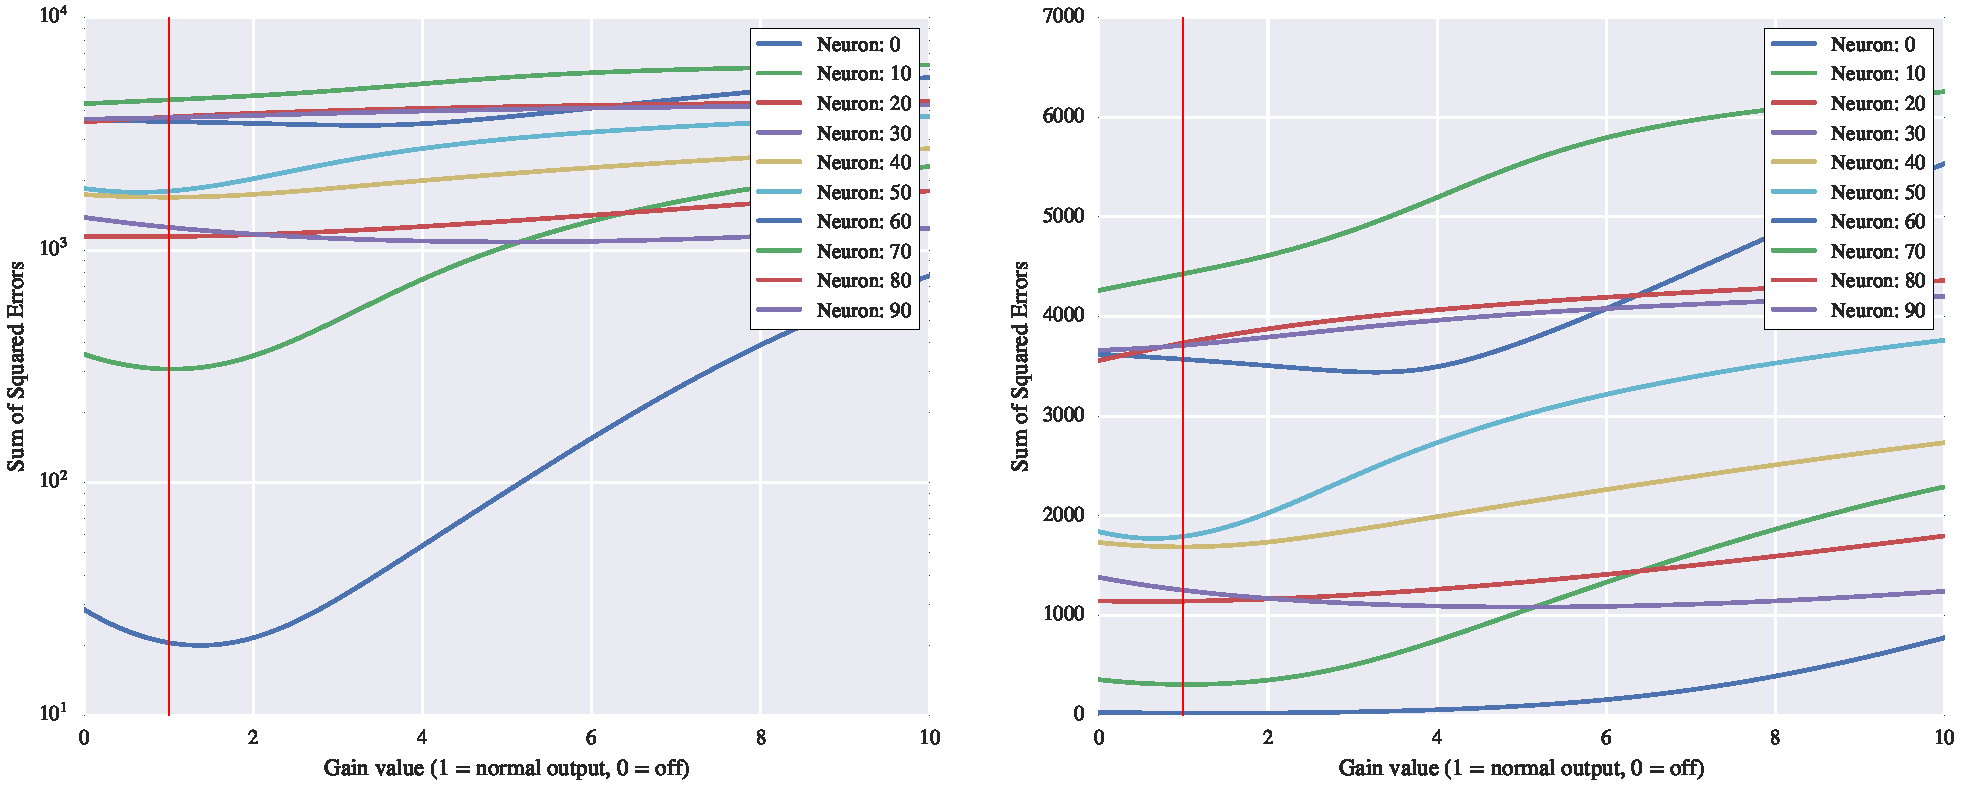
\includegraphics[width=\linewidth]{png/mnist-deep-g2-gain.pdf}
\caption{Error surface of the network output in log space (left) and in real space (right) with respect to each candidate neuron chosen for removal using the 2nd order Taylor Series error approximation criterion; (\textbf{Network:} 2 layers, 50 neurons/layer, 10 outputs, logistic sigmoid activation, starting test accuracy: 1.000)}
\label{fig:mnist-g2-double-layer}
\end{figure}


As seen in the case of a single layered network, these graphs are a visualization the error surface of the network output with respect to the neurons chosen for removal using each algorithm, represented in intervals of 10 neurons. 

\textbf{Brute Force Criterion}

It is clear why these neurons got chosen, their graphs clearly show little change when neuron is removed, are mostly near the floor, and show convex behaviour of error surface, which argues for the rationalization of using 2nd order methods to estimate difference in error when they are turned off.

\textbf{1st Order Approximation Criterion}

Drawing a flat line at the point of each neurons intersection with the red vertical line (no change in gain) shows that the 1st derivative method is actually accurate for estimation of change in error in these cases, but still ultimately leads to poor decisions. 

\textbf{2nd Order Approximation Criterion}

Clearly these neurons are not overtly poor candidates for removal (error doesn't change much between 1.0 \& zero-crossing left-hand-side), but could be better (as described above in the Brute Force Criterion discussion).


\subsection{Experiments on Toy Datasets}

As can be seen from the experiments on MNIST, even though the 2nd-order approximation criterion is consistently better than 1st-order, it's performance is not nearly as good as brute force based ranking, especially beyond the first layer. What is interesting to note is that from some other experiments conducted on toy datasets (predicting whether a given point would lie inside a given shape on the Cartesian plane), the performance of the 2nd-order method was found to be exceptionally good and produced results very close to the brute force method. The 1st-order method, as expected, performed poorly here as well. Some of these results are illustrated in Figure \ref{fig:diamond}. 

\begin{figure}[!hb]
\centering
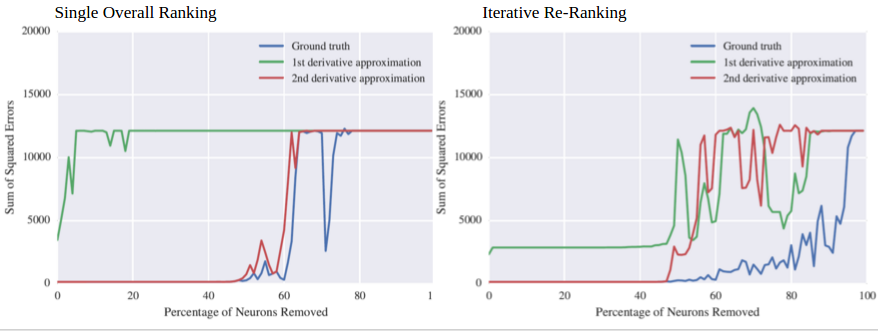
\includegraphics[width=0.80\linewidth]{png/diamond.png}
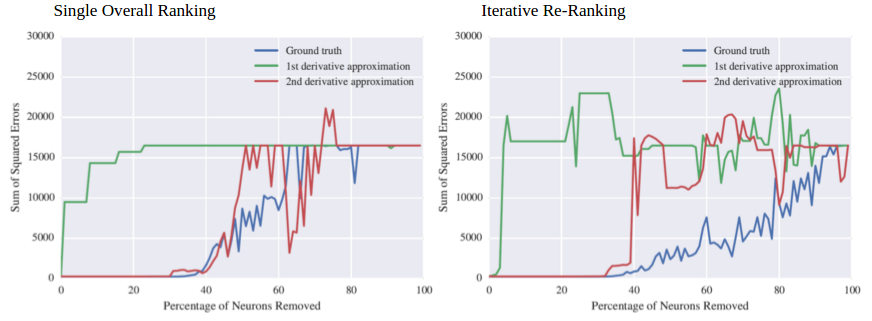
\includegraphics[width=0.80\linewidth]{png/rshape.png}
\caption{Degradation in squared error after pruning a 2-layer network using the Single Pass Algorithm (left) and the Iterative Re-ranking algorithm(right) on toy "diamond" shape dataset (above) and toy "random shape" dataset (below); (\textbf{Network:} 2 layers, 50 neurons/layer, 10 outputs, logistic sigmoid activation, starting test accuracy: 0.992(diamond); 0.986(random shape)}
\label{fig:diamond}
\end{figure}

%This huge variation in results from MNIST might be attributed to the fact that these toy datasets had only 2 output classes (as opposed to 10 classes in MNIST), but it certainly warrants further investigation.